\documentclass[a4paper, 12pt]{article}
\usepackage[left = 13 mm, top = 15mm, right = 13 mm, bottom = 23mm, bindingoffset = 7mm]{geometry}
\usepackage[T2A,T1]{fontenc}
\usepackage[utf8]{inputenc}
\usepackage[english,russian]{babel}
\usepackage{graphicx}
\usepackage{amssymb, mathtools}
\usepackage{lipsum}
\usepackage{float}
\usepackage{wrapfig}
\usepackage{indentfirst} 
\usepackage{icomma}

\newcommand{\HRule}{\rule{\linewidth}{0.3mm}}

\newcommand{\LabTitle}{Измерение удельного заряда электрона}
\begin{document}




\begin{titlepage}
\begin{center}\large
ФГАУ ВПО <<МОСКОВСКИЙ ФИЗИКО-ТЕХНИЧЕСКИЙ УНИВЕРСИТЕТ>>
\begin{figure}[H]
\centering

\includegraphics[width=15cm]{logo.jpg}
\end{figure}
{\Large
Кафедра радиотехники}

\vfill

\hrule
\vspace{0.3cm}

\huge \LabTitle

\vspace{0.3cm}
\hrule


%\noindent\rule{\textwidth}{0.4mm}
%\huge Магнитометр
%\noindent\rule{\textwidth}{0.4mm}


\end{center}

\vfill


\begin{minipage}{0.7\textwidth}
\textbf{Выполнил:}
Корепанов Г.М.

512 группа

\vspace{0.5cm}

\textbf{Преподаватель:}
Филатов Иван Васильевич
\end{minipage}


\vfill
\centering
 Долгопрудный, 2016 г.




\end{titlepage}


\section*{Экспериментальная установка №~1}
\begin {wrapfigure}[23]{l}{0.4\textwidth}
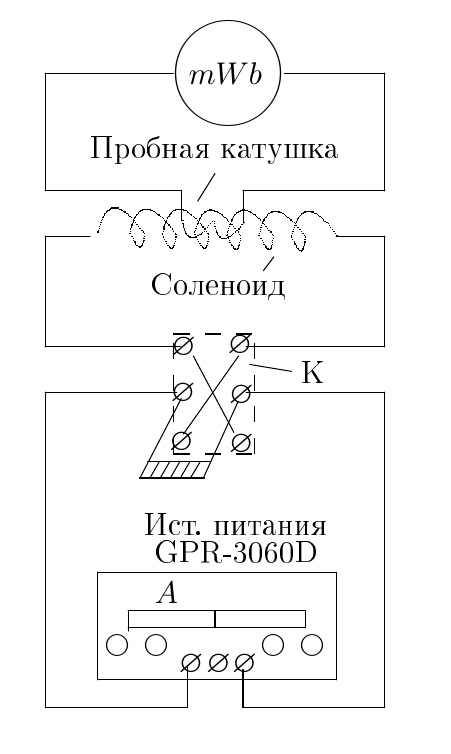
\includegraphics[trim=0 0 0 20,clip,width=\linewidth]{eq1}
\caption{Схема установки}
\end {wrapfigure}
\textbf{Параметры установки}
\begin{gather*}
l=26,5 \text{ см}\\
SN=3000 \text{ см}^2\\
r_\text{out}=5 \text { Ом}
\end{gather*}

\section*{Магнитная фокусировка, теория}
Электрон, влетающий в однородное магнитное поле, движется по ларморовской окружности (сила Лоренца перпендикулярна скорости и обеспечивает центростремительное ускорение), радиус которой зависит от модуля скорости, а частота -- нет:
\begin{equation}
T = \frac{2\pi m}{eB} \label{a}
\end{equation}
Если запустить пучок электронов с разной поперечной скоростью, но одинаковой продольной (это как раз и обеспечивает подача переменного напряжения на отклоняющие пластины), то электроны, двигаясь по спиралям разного радиуса, на расстояниях $L = n\cdot T\mu_{||}$ будут собираться в пучки, поскольку каждый из них через время, равное периоду обращения по окружности, вернется на изначальную ось, а расстояния, которое электроны пройдут за время, равное этому периоду, будут совпадать в силу равенства начальных продольных скоростей $\nu_{||}$.

Продольную скорость можно выразить через ускоряющее напряжение ЭЛТ:
$$eV = \frac{m\nu^2}{2},$$
подставляя скорость в (\ref{a}), получим выражение для удельного заряда электрона:
$$\frac{e}{m} = \frac{8\pi^2 V}{l^2} \frac{n^2}{B^2},$$
то есть зависимость между $B$ и $n$ при постоянной длине ЭЛТ $l$ является линейной.

\pagebreak
\section*{Экспериментальная установка №~2}
\begin {wrapfigure}[17]{l}{0.6\textwidth}
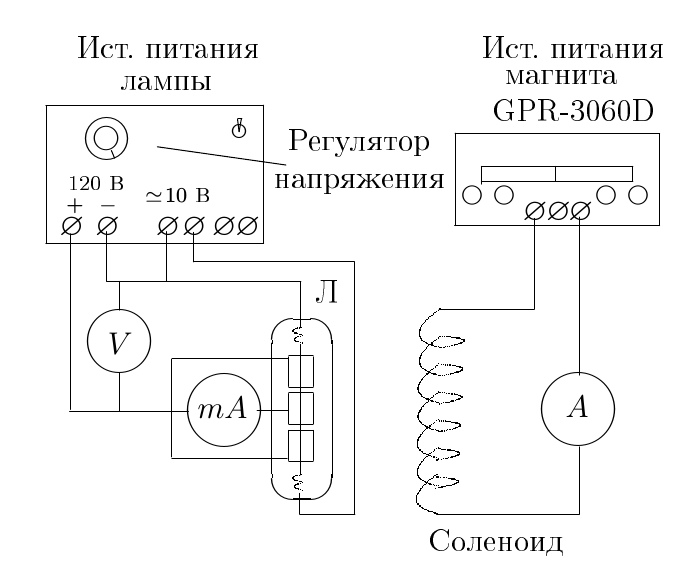
\includegraphics[trim=0 0 0 20,clip,width=\linewidth]{eq2}
\caption{Схема установки}
\end {wrapfigure}
\textbf{Параметры установки}
\begin{gather*}
l=26,5 \text{ см}\\
SN=3000 \text{ см}^2\\
r_\text{out}=5 \text { Ом}
\end{gather*}

\section*{Метод магнетрона, теория}
Электроны, вылетающие с катода двухэлектродной лампы, летят по радиусу (эл. поле радиально) к внешнему цилиндру -- аноду. Включение внешнего магнитного поля искривляет траекторию -- тем сильнее, чем больше величина магнитного поля. При некотором критическом значении поля электроны перестану достигать анода, возвращаясь по кривой к аноду. 

Уравнение движения электронов в таком поле легко получить, записывая уравнение моментов в цилиндрических координатах:

\begin{gather*}
F_\varphi^{\text{маг}} = e\nu_rB, \quad F_r^{\text{маг}} = -e\nu_\varphi B\\
F_r^{\text{эл}} = eE
\end{gather*}

Поскольку момент импульса в полярных координатах записывается как
$$L=mr^2\dot{\varphi}$$

Отсюда с учетом начальных условий (электрон вылетает с очень тонкого катода с почти нулевой начальной скоростью) получим
$$r^2\dot{\varphi} = \frac{eBr^2}{2m}$$
Используя закон сохранения энергии, получим окончательный результат:

$$eV=\frac{m}{2}\left[\dot{r}^2+\left(\frac{eBr}{2m}\right)^2\right]$$
Уравнение для $B_\text{кр}$ найдем, используя, что радиальная скорость электрона при достижении анода ($r=r_{\text{а}}$) равна 0 ($\dot(r) = 0$):
$$\frac{e}{m}=\frac{8V_\text{а}}{B_\text{кр}^2 r_\text{а}^2}$$



\pagebreak
\section*{Эксперимент №~1}
Откалибруем соленоид, измерив зависимость магнитного поля от тока, через него протекающего:
\begin {figure}[H]
\begin{center}
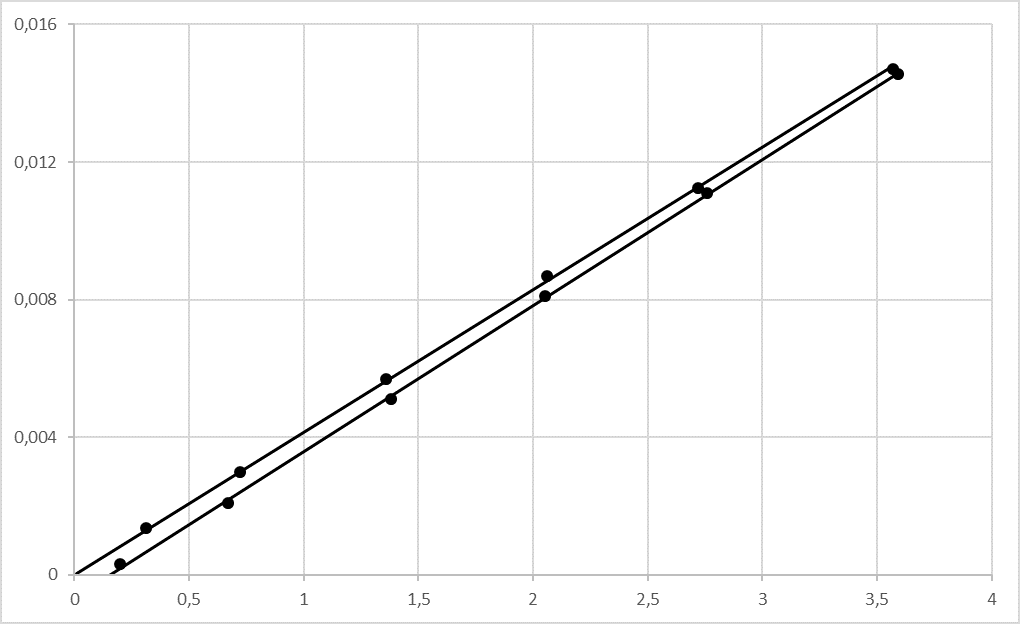
\includegraphics[width=\textwidth]{graph1_gk}
\caption{Зависимость $B=f(I)$}
\end{center}
\end {figure}


Усредненное значение коэффициента пропорциональности между полем и током:
$$K = (4,19 \pm 0,15) \frac{\text{мТл}}{\text{А}}$$

Зная поле для произвольного тока, можем снять зависимость поля в соленоиде от порядка фокусировки:
тока, через него протекающего:
\begin {figure}[H]
\begin{center}
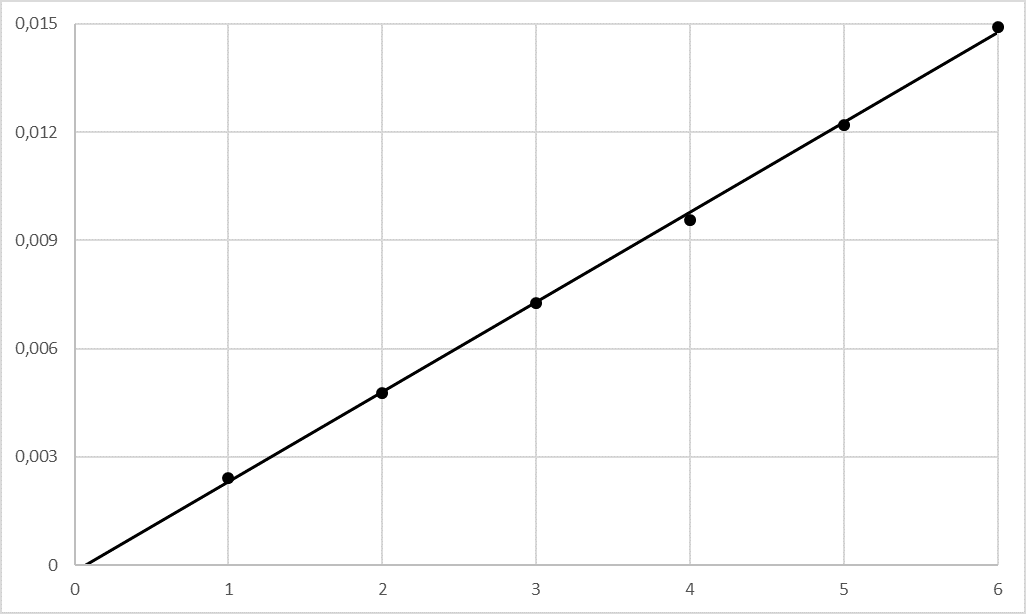
\includegraphics[width=\textwidth]{graph2_gk}
\caption{Зависимость $B=f(n)$}
\end{center}
\end {figure}



По наклону графика определяем удельный заряд электрона:
$$\frac{e}{m} = (1,71\pm 0,07) \cdot 10^{11} \frac{\text{Кл}}{\text{кг}}$$



\pagebreak
\section*{Эксперимент №~2}
Семейство кривых $\mathbf{I_\text{а}(B)}$ для разных значений анодного напряжения $V_\text{а}$:


\begin {figure}[H]
\begin{center}
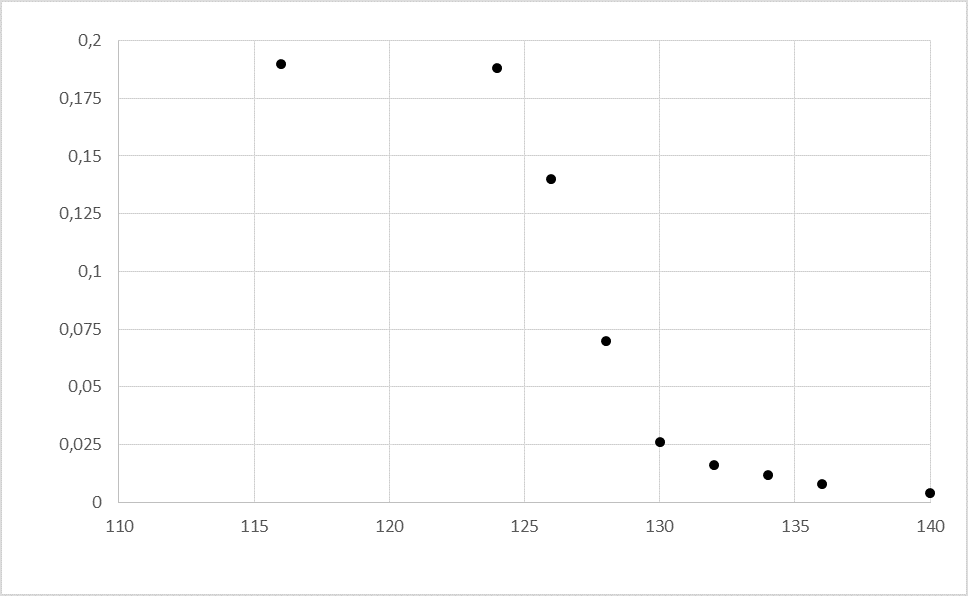
\includegraphics[width=0.95\textwidth]{graph3_gk}
\caption{Зависимость анодного тока от магнитного поля для $V_\text{а}=60$ В}
\end{center}
\end {figure}



\begin {figure}[H]
\begin{center}
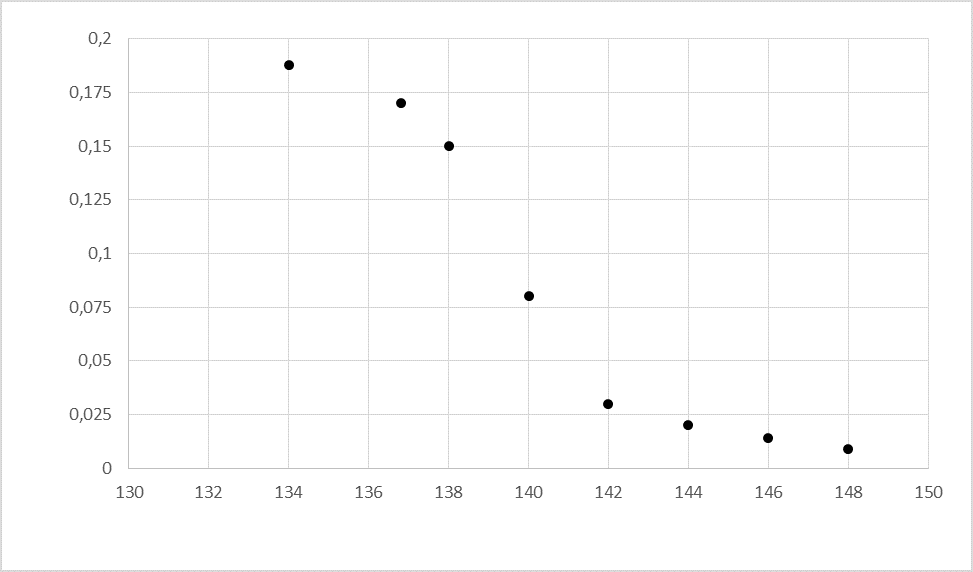
\includegraphics[width=0.95\textwidth]{graph4_gk}
\caption{Зависимость анодного тока от магнитного поля для $V_\text{а}=85$ В}
\end{center}
\end {figure}



\begin {figure}[H]
\begin{center}
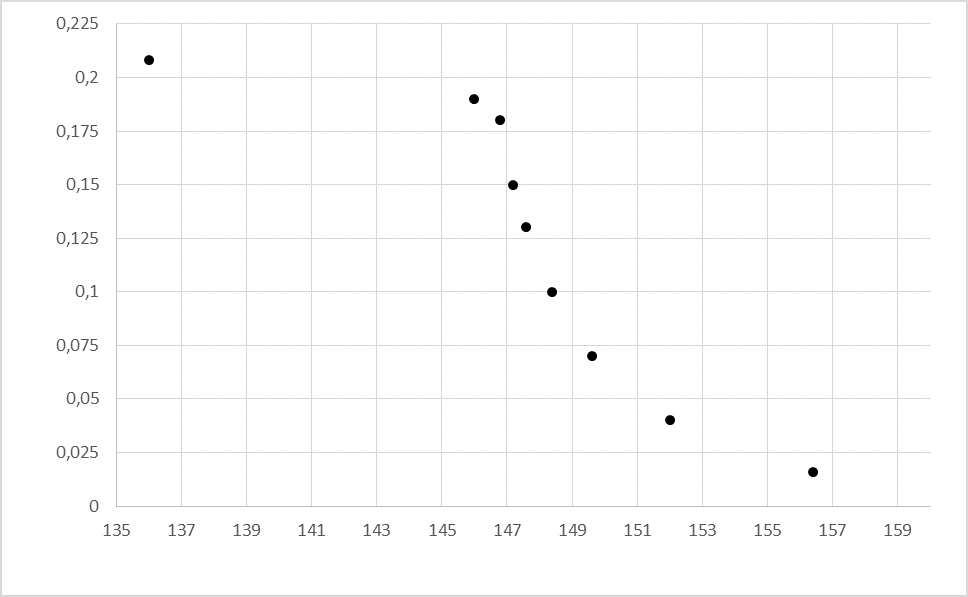
\includegraphics[width=0.95\textwidth]{graph5_gk}
\caption{Зависимость анодного тока от магнитного поля для $V_\text{а}=100$ В}
\end{center}
\end {figure}



\begin {figure}[H]
\begin{center}
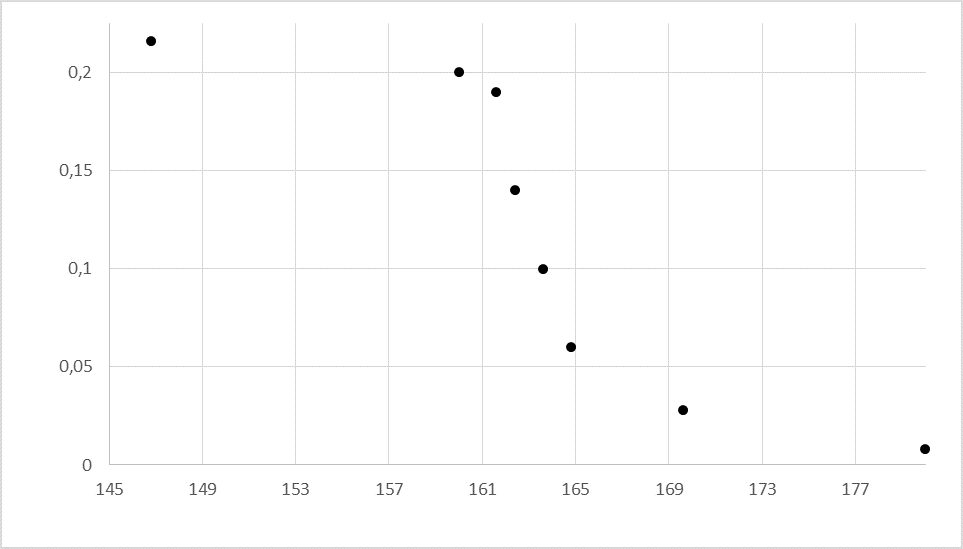
\includegraphics[width=0.95\textwidth]{graph6_gk}
\caption{Зависимость анодного тока от магнитного поля для $V_\text{а}=120$ В}
\end{center}
\end {figure}




\newpage
Соберем полученные значения критических полей в одну таблицу:

\begin{table}[H] 
\centering 
\begin{tabular}{|l|l|l|l|l|} 
\hline 
\textbf{$V_\text{а}$} & 60 & 85 & 100 & 120 \\ \hline 
\textbf{$B_\text{кр}$} & 4,445 & 4,8825 & 5,187 & 5,6875 \\ \hline 
\end{tabular} 
\caption{Зависимость критического поля от анодного напряжения} 
\label{my-label} 
\end{table}


По полученным значениям строим график $B_\text{кр}^2(V_\text{а})$:

\begin {figure}[H]
\begin{center}
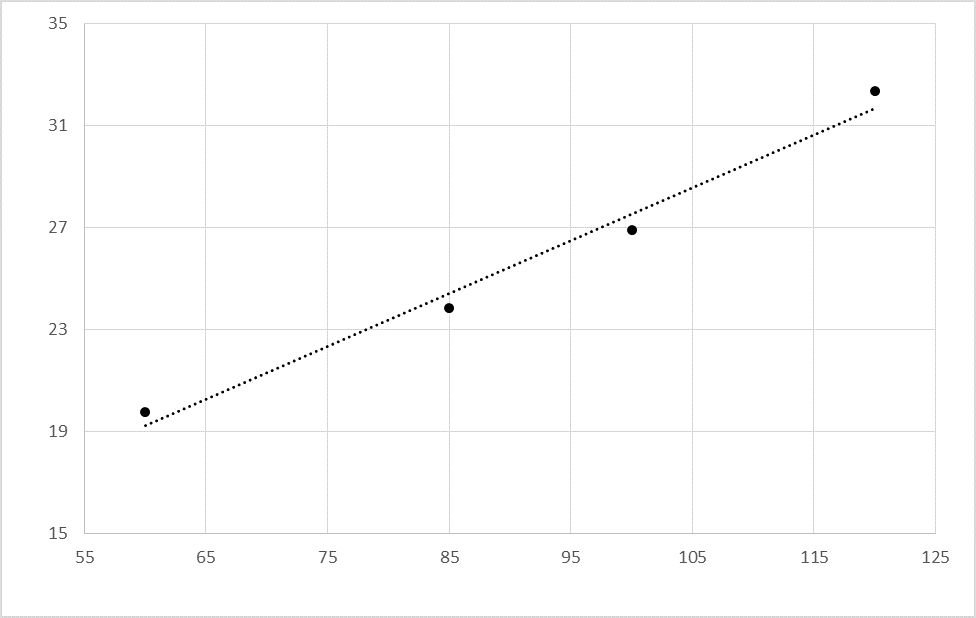
\includegraphics[width=\textwidth]{graph7_gk}
\caption{Зависимость квадрата критического значения поля от анодного напряжения}
\end{center}
\end {figure}
По наклону графика определяем удельный заряд электрона:
$$\frac{e}{m} = (1,82 \pm 0,17) \cdot 10^{11} \text{ Кл/кг}$$

\end{document}